\documentclass[tikz,border=10pt]{standalone}
\usepackage{tikz}
\usetikzlibrary{calc,patterns,decorations.pathreplacing,arrows.meta}

\begin{document}

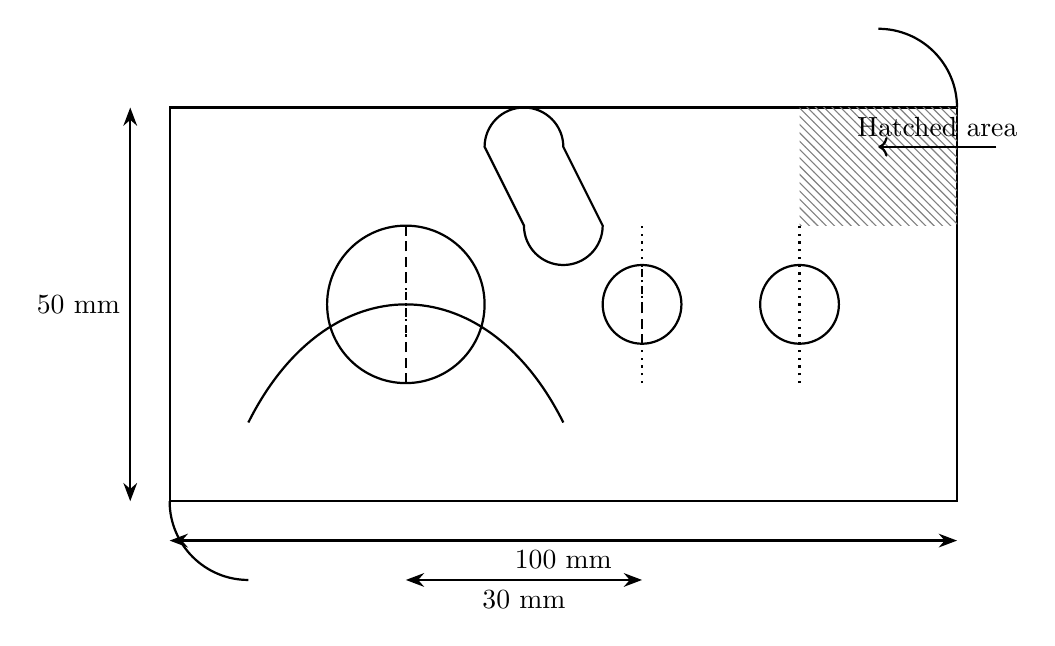
\begin{tikzpicture}
    % Styles
    \tikzset{
        dimline/.style={thick, >=Stealth, <->},
        hidden/.style={dashed, thick},
        centerline/.style={dotted, thick},
        hatching/.style={pattern=north west lines, pattern color=black!50},
        filled/.style={fill=black!20}
    }

    % Main base
    \draw[thick] (0,0) rectangle (10,5);

    % Large hole
    \draw[thick] (3,2.5) circle (1);

    % Smaller holes
    \foreach \x in {6,8}
        \draw[thick] (\x,2.5) circle (0.5);

    % Fillets (rounded corners)
    \draw[thick] (10,5) arc[start angle=0, end angle=90, radius=1];
    \draw[thick] (0,0) arc[start angle=180, end angle=270, radius=1];

    % Slot (oblong hole)
    \draw[thick] (5,4.5) arc[start angle=0, end angle=180, radius=0.5] -- (4.5,3.5) arc[start angle=180, end angle=360, radius=0.5] -- cycle;

    % Bezier curve
    \draw[thick] (1,1) .. controls (2,3) and (4,3) .. (5,1);

    % Center marks
    \foreach \x in {3,6,8}
        \draw[centerline] (\x,1.5) -- (\x,3.5);

    % Hatching (Cross-sectioned area)
    \fill[hatching] (8,3.5) rectangle (10,5);

    % Hidden lines
    \draw[hidden] (3,1.5) -- (3,3.5);
    \draw[hidden] (6,2) -- (6,3);
    
    % Dimensioning
    \draw[dimline] (0,-0.5) -- (10,-0.5) node[midway, below] {100 mm};
    \draw[dimline] (-0.5,0) -- (-0.5,5) node[midway, left] {50 mm};
    \draw[dimline] (3,-1) -- (6,-1) node[midway, below] {30 mm};
    
    % Section indicators
    \draw[thick, ->] (10.5,4.5) -- (9,4.5) node[midway, above] {Hatched area};

\end{tikzpicture}

\end{document}
